\begin{figure}[!ht]
    \centering
    a)
    \begin{minipage}{.45\textwidth}
        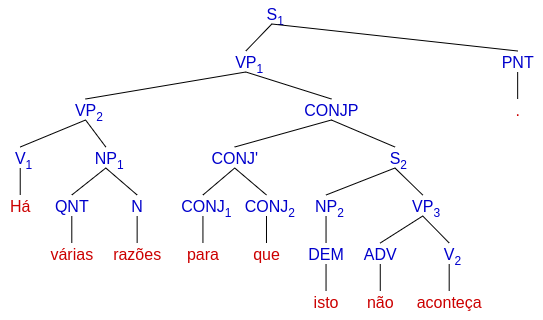
\includegraphics[width=\linewidth]{imagens/ec_cintil_conjp_tree_orig.png}
    \end{minipage}
    \hfill
    b)
    \begin{minipage}{.45\textwidth}
        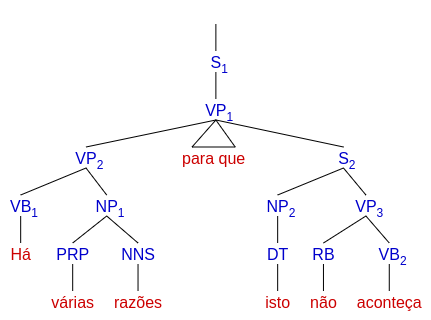
\includegraphics[width=\linewidth]{imagens/ec_cintil_conjp_tree_trans.png}
    \end{minipage}
    \hfill
    \vskip\floatsep
    c)
    \begin{minipage}{.45\textwidth}
        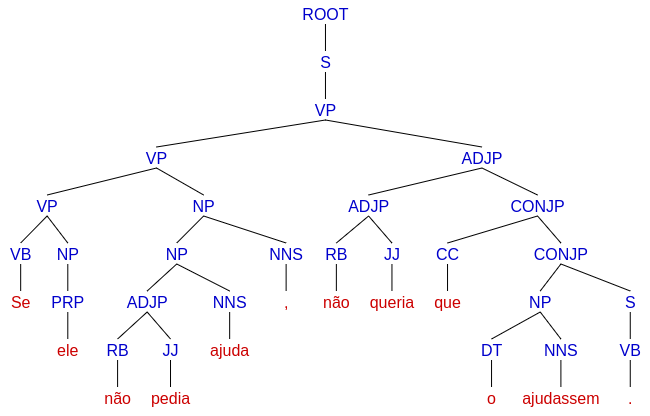
\includegraphics[width=\linewidth]{imagens/ec_cintil_conjp_tree_sp.png}
    \end{minipage}
    \caption[Estudo de caso CINTIL - Árvore da sentença transduzida com CONJP]{Estudo da sentença eCTMP-001150/117736, \textquote{Há várias razões para que isto não aconteça.}, que possui CONJP internamente. Em a), temos a árvore como se apresenta originalmente no CINTIL. Em b), temos a mesma sentença, pós transdução. Em c), temos o resultado da classificação do SP, utilizando a gramática gerada neste trabalho (após o processo de transdução)}
    \label{fig:ec_cintil_conjp_tree}
\end{figure}